\chapter{Analisis}
\label{chap:analysis}
Pada bab ini, akan dijelaskan mengenai analisis Input dan fitur perangkat lunak, Diagram pengembangan perangkat lunak, \textit{use case} dari perangkat lunak serta diagram aktifitas dari perangkat lunak.
\section{Analisis Input}
\subsection{Analisis File Excel Jadwal Mengawas Ujian}
Sub bab ini akan membahas analisis file excel yang dikeluarkan oleh TU.\\
TU FTIS mengeluarkan jadwal setiap tahunnya yang dibagikan kepada dosen FTIS. 
berikut ini contoh file excel yang dikeluarkan oleh TU. 
\begin{figure}[H]
	\centering
	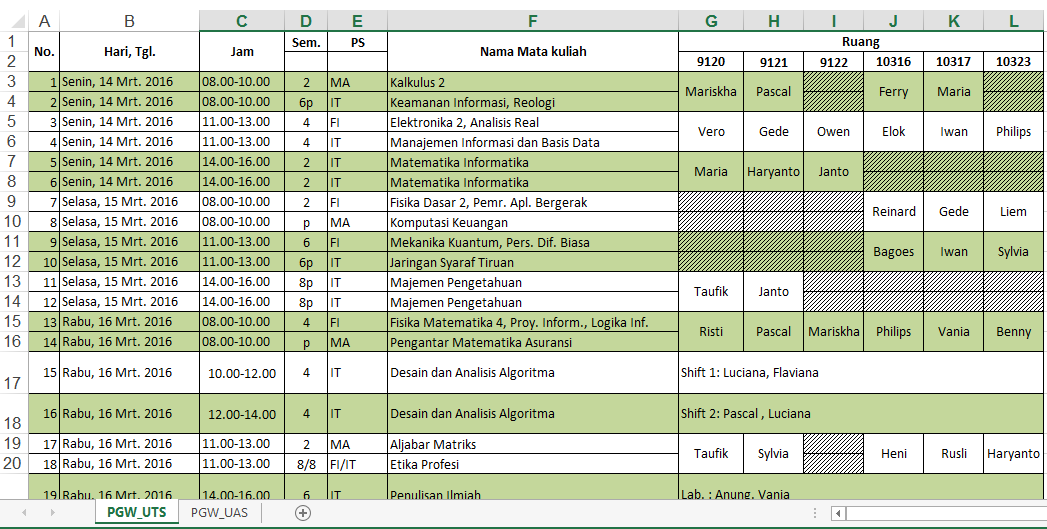
\includegraphics[scale=0.5]{Gambar/scJadwal}
	\caption{Jadwal mengawas ujian FTIS}
	\end{figure}
	
Berikut penjelasan kolom-kolom yang ada di gambar \textbf{3.1}\\
\begin{tabular}{|c|p{12cm}|}
		\hline
		\textbf{No} & \textbf{Kolom dan Deskripsi} \\ \hline \hline
		1 & \textbf{No}\\
			&	Menyatakan nomer urut jadwal mengawas ujian.\\ \hline
		2 & \textbf{Hari, Tanggal}\\
			&	Kolom dalam bentuk String berisi hari dan tanggal. Terdapat singkatan yang diberikan TU dalam contoh ini  Mrt. menunjukan bulan Maret\\ \hline	
		3 & \textbf{Jam}\\
			&	Kolom ini bertipe String dan menerangkan pukul dilaksakannya ujian.\\ \hline
		4 & \textbf{Semester}\\
			&	Kolom ini bertipe String dan mengerangkan semester dari mata kuliah yang di ujiankan . Terdapat simbol p yang menerangkan matakuliah pilihan\\ \hline
		5 & \textbf{PS}\\
			&	Bertipe string berisi jurusan yang ujian mata kuliah tersebut.\\ \hline
		6 & \textbf{Nama Mata Kuliah}\\
			&	Kolom bertipe String dan berisi tentang mata kuliah yang di ujiankan.\\ \hline
		7 & \textbf{Ruangan}\\
			&	Kolom dengan merge 6 kolom dan pada baris kedua terdapat 6 kolom ruangan ujian yaitu 9120, 9121, 9122, 10316, 10317, 10323. Masing kolom kelas berisi nama dosen yang mengawas bertipe String. Ruangan tidak terpakai ditandai dengan garis-garis miring. Jika ada isi kolom kelas yang dimerge sebanyak 6 kolom menandakan kelas tersebut adalah lab.\\ \hline
	\end{tabular}	
	\\
Dari gambar \textbf{3.1} terpilih beberapa kolom untuk dapat ditampilkan pada PL, Berikut analisanya :\\
\begin{tabular}{|c|p{12cm}|}
		\hline
		\textbf{No} & \textbf{Kolom dan Deskripsi} \\ \hline \hline
		1 & \textbf{Hari, Tanggal}\\
			&	Kolom ini bertipe String dan terdapat singkatan seperti Mrt, maka akan dibuatkan fungsi pada saat implementasi agar seragam dan sesuai dengan format tgl dan waktu pada Java.\\ \hline	
		2 & \textbf{Jam}\\
			&	Kolom ini bertipe String, maka dibutuhkan konversi String kedalam fungsi jam pada saat implementasi.\\ \hline
		3 & \textbf{Nama Mata Kuliah}\\
			&	Kolom ini dapat menerangkan deskripsi mata kuliah pada PL.\\ \hline
		4 & \textbf{Owner}\\
			&	Kolom ini merupakan isi dari tabel kelas pada excel, pada PL akan ditampilkan sebagai kolom tersendiri menerangkan Dosen yang mengawas matakuliah.\\ \hline		
		7 & \textbf{Ruangan}\\
			&	Kolom ini akan berisi kelas sesuai dosen yang mengajar, mata kuliah, waktu dan tanggal.\\ \hline
	\end{tabular}

\subsection{Analisis Fitur Perangkat Lunak}
Perangkat Lunak ini akan memiliki fitur sebagai berikut : 
	\begin{enumerate}
		\item \textit{Tool} ini dapat menerima dan membaca\textit{input} file excel jadwal mengawas ujian yang dikeluarkan TU FTIS.
		\item \textit{Tool} ini dapat mengubah file excel menjadi iCalendar.
		\item File iCalendar dapat di unduh oleh pengguna.
		\item Pengguna dapat melakukan \textit{sort} sesuai dengan nama yang di inginkan.
	\end{enumerate}
	
\section{Permodelan Tool}

Berikut diagram use case berserta skenario yang tertera pada gambar \textbf{3.2}

\begin{figure}[h]
	\centering
	\includegraphics[scale=0.5]{Gambar/useCaseJadwal}
	\caption{Diagram use case \textit{tool} konversi jadwal mengawas ujian}
	\end{figure}

\begin{enumerate}
	\item Skenario Memasukan input file excel \\
	{\renewcommand\labelitemi{}
		\begin{itemize}
			\item Deskripsi		: Kegiatan memasukan input file excel.
			\item Aktor				: Dosen
			\item Prakondisi	: -
			\item Skenario		:
				\begin{itemize}
					\item Dosen memasukan file excel mengawas ujian yang keluarkan oleh TU
				\end{itemize}
		\end{itemize}
		}
		
	\item Skenario Melakukan Sorting nama
	{\renewcommand\labelitemi{}
	\begin{itemize}
			\item Deskripsi		: Kegiatan mensorting jadwal mengawas.
			\item Aktor				: Dosen
			\item Prakondisi	: -
			\item Skenario		:
				\begin{itemize}
					\item Dosen dapat melakukan sorting nama dari jadwal ujian yang telah berupa iCal sesuai nama yang di inginkan. 
				\end{itemize}
		\end{itemize}
		}
		
		\item Skenario Mengunduh File iCal 
		{\renewcommand\labelitemi{}
		\begin{itemize}
			\item Deskripsi		: Kegiatan Mengunduh file iCal.
			\item Aktor				: Dosen 
			\item Prakondisi	: -
			\item Skenario		:
				\begin{itemize}
					\item Dosen mengunduh file iCal yang telah dikonversi oleh \textit{tool}
				\end{itemize}
		\end{itemize}
		}
\end{enumerate}

\section{Diagram Aktifitas}
Pada subbab ini akan dibahas mengenai prosedur setiap aktifitas dari fitu yang diberikan oleh \textit{tool}.

\subsection{Memasukan Excel Jadwal Mengawas Ujian}
Tahap ini merupakan tahap awal proses file input dimasukan kedalam program dimana file input yang dimaksud merupakan excel jadwal yang dikeluarkan TU FTIS. Berikut step-step untuk memasukan excel kedalam program.
\begin{figure}[h]
	\centering
	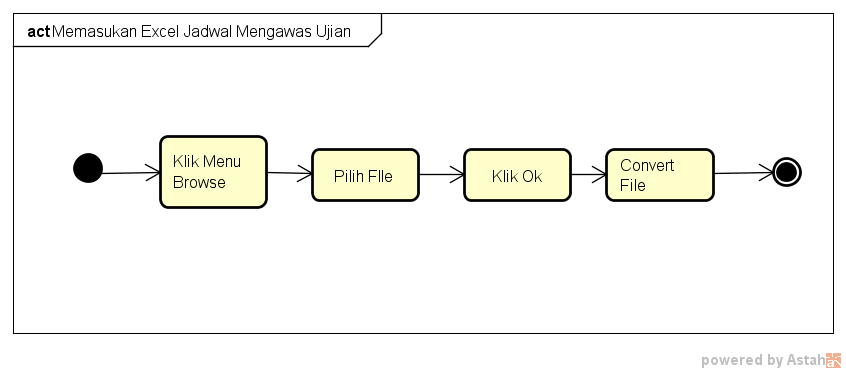
\includegraphics[scale=0.5]{Gambar/Memasukan-Excel-Jadwal-Mengawas-Ujian}
	\caption{Prosedur Memasukan Excel Jadwal Mengawas Ujian}
	\end{figure}
	
\begin{enumerate}
	\item Pengguna mengklik menu Browse yang ada di program. 
	\item Pengguna memilih file yang akan dimasukan.
	\item Pengguna mengklik tombol oke pada window.
	\item Pengguna dapat mengklik tombol Convert untuk mengkonversi file excel menjadi iCal.
\end{enumerate}

\subsection{Sorting Nama Dosen}
Tahap ini menjelaskan bagaimana pengguna dapat memanfaatkan fitur dari program dengan mensorting nama dosen, dengan begitu jadwal dosen yang dicari dapat di unduh dengan mudah. Berikut step-step untuk mensorting nama dosen.
\begin{figure}[H]
	\centering
	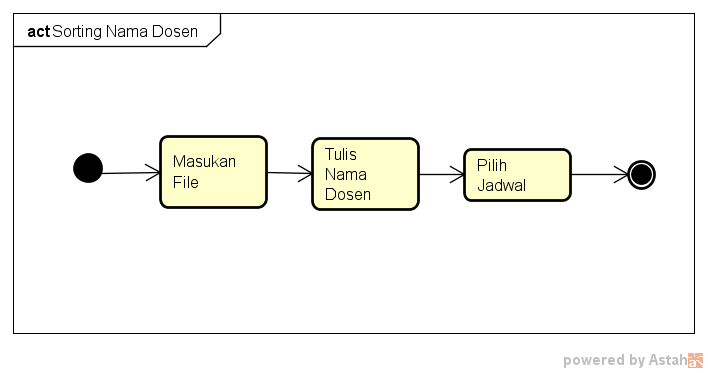
\includegraphics[scale=0.5]{Gambar/Sorting-Nama-Dosen}
	\caption{Prodsedur Sorting Nama Dosen}
	\end{figure}

\begin{enumerate}
	\item Syarat dari penggunaan sorting adalah file harus dimasukan lalu di konversu terlebih dahulu .
	\item Setelah file dikonversi, pengguna dapat memasukan nama dosen dicari dengan mengetikan nama pada kolom filter by owner.
	\item Setelah pengguna mengetikan nama lalu muncul nama dosen dicari, pengguna dapat mengunduh jadwal sesuai pilihan.
\end{enumerate}

\subsection{Unduh File iCal}
Tahap ini merupakan tahap terakhir, file excel yang telah dimasukan lalu dikonversi menjadi iCal selanjutnya pengguna tinggal memilih jadwal mana yang akan di unduh. File iCal yang telah di konversi tersebut dapat di integrasikan dengan \textit{paltform} lain seperti google calendar, apple iCal, dll. Berikut step-step untuk mengunduh file iCal.
\begin{figure}[h]
	\centering
	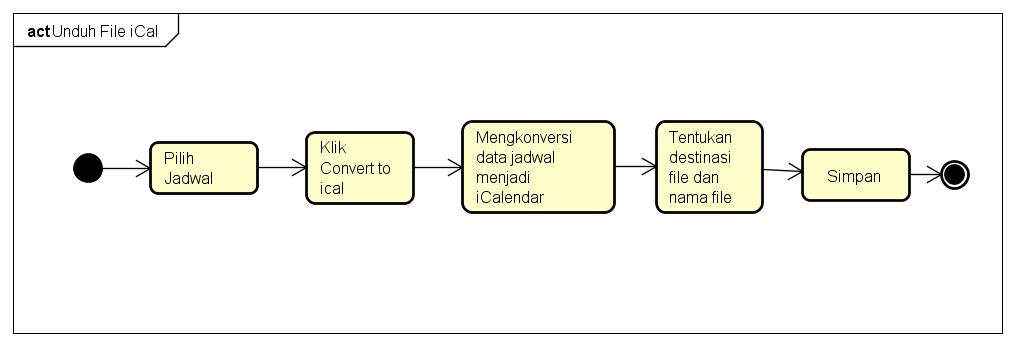
\includegraphics[scale=0.5]{Gambar/Unduh-File-iCal}
	\caption{Prosedur Mengunduh File iCal}
	\end{figure}

\begin{enumerate}
	\item Sebelum mengunduh pengguna diwajibkan mengkonversi terlebih dahulu file jadwal mengawas dengan mengklik tombol Convert pada program.
	\item Setelah di konversi, pengguna dapat memilih jadwal yang akan di unduh.
	\item Setelah itu, pengguna mengklik tombol iCal pada jadwal dipilih.
	\item Akan muncul Pop-Up untuk konfirmasi menyimpan, kemudian klik tombol simpan untuk menyimpan file iCal.
\end{enumerate}